%% notes-tex/026-kinetics-thermodynamics/sections/4-reproduction.tex
%% [[experiments.026-metabolism-flux.scripts.plot_kinetic_distributions]]
%% https://github.com/Mjvolk3/torchcell/tree/main/notes-tex/026-kinetics-thermodynamics/sections/4-reproduction.tex

\section{Reproducing Wu et al.'s Fig.~3\secstatus{todo}}

\subsection{What the original figure claims\secstatus{todo}}

Wu et al. (2026) build Yeast-MetaTwin, a comprehensive metabolic network for
\emph{S.~cerevisiae} obtained by expanding reaction rules over the yeast metabolome, and
ask how the resulting \emph{underground} reactions differ kinetically from the
\emph{core} network already in Yeast9. Their Fig.~3a--h answers it with eight empirical
cumulative distributions, one per predictor and parameter: $k_{cat}$ from DLKcat, UniKP,
EITLEM-Kinetics, TurNuP and DeepEnzyme, then $K_M$ from Boost\_KM, UniKP and
EITLEM-Kinetics. Their conclusion is that underground metabolism is separated from known
metabolism by $K_M$ rather than by $k_{cat}$.

The construction is taken from their own notebook: sort the values, plot the running
proportion, and mark each curve's median with a short vertical tick. Their split is on
whether a reaction identifier contains \texttt{rxn}, which is how their tables encode a
predicted rather than a curated reaction.

\subsection{The per-pair predictions behind Fig.~3 were not released\secstatus{todo}}

The intention was to draw two things on each panel: the authors' own released predictions
split core against underground, and our independent re-run over yeast-GEM. The first is not
available.

Their notebook reads its tables from \texttt{Results/kcat\_km\_predict/}, naming each one
explicitly:

\begin{itemize}\setlength{\itemsep}{0pt}
  \item \texttt{yeast8U\_kcat\_predict.csv} \quad DLKcat
  \item \texttt{yeast8U\_unikp.csv} \quad UniKP, both parameters
  \item \texttt{yeast8U\_kcat\_result\_TurNuP.csv} \quad TurNuP
  \item \texttt{yeast8U\_km\_km\_predict.csv} \quad Boost\_KM
\end{itemize}

\noindent That directory is in neither released artifact. The GitHub repository ships \texttt{Results/} with nine subdirectories, none of
them \texttt{kcat\_km\_predict}, and its \texttt{source\_data} holds only
\texttt{fig2-a}, \texttt{fig3-g}, \texttt{fig3-j}, \texttt{fig4-b}, \texttt{fig5-b},
\texttt{figs11} and \texttt{figS8}; the file named \texttt{fig3-g.csv} contains EC-number
counts rather than a $K_M$ distribution. The 6.6 GB Zenodo archive
(10.5281/zenodo.13911783) contains exactly three top-level directories, \texttt{Data},
\texttt{Data\_retrosynthesis} and \texttt{esm}, and of its 1{,}021{,}022 entries
\textbf{zero} match \texttt{kcat}, \texttt{unikp}, \texttt{turnup}, \texttt{eitlem} or
\texttt{deepenzyme}.

This is checkable and is stated as a fact about the release rather than as a criticism of
the work: the Data Availability statement says data for reproducing all figures is
available on GitHub and Zenodo, and for Fig.~3a--h it is not.

Two consequences follow. The \textbf{underground arm cannot be drawn}, because generating
the Yeast-MetaTwin reaction set is a separate retrobiosynthesis pipeline that this work
does not rebuild. And what remains is the stronger half of a reproduction anyway: the
curves in Figure~\ref{fig:kinetics-fig3} are re-derived by running the same published
models over the same organism from hash-pinned mirrors, rather than re-plotted from
someone else's numbers.

\begin{figure}[H]
  \centering
  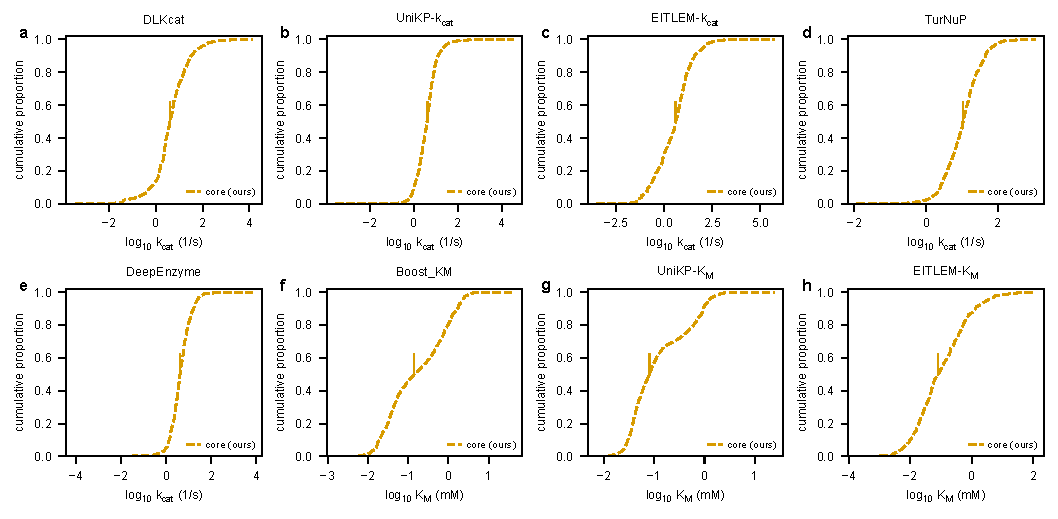
\includegraphics[width=\textwidth]{figures/kinetics_fig3.pdf}
  \caption[Predicted kinetic parameter distributions, after Wu et al. Fig.~3a--h]{Empirical
  cumulative distributions of predicted kinetic parameters, following Wu et al. (2026)
  Fig.~3a--h. Panels a--e are $k_{cat}$, panels f--h are $K_M$; the predictor is named on
  each panel. Amber dashed is our independent run of the same predictor over yeast-GEM
  9.0.2, which is the core network. The authors' core and underground curves are absent
  because the per-pair tables their notebook reads are in neither released artifact, as
  the text sets out. A short vertical tick marks each curve's median, as in the original.
  All eight predictors ran, so every panel carries a curve. Generated
  by
  \texttt{experiments/026-metabolism-flux/scripts/plot\_kinetic\_distributions.py}.}
  \label{fig:kinetics-fig3}
\end{figure}

\subsection{The log base is not a convention\secstatus{todo}}

Each predictor was validated against something its own authors published, and the exercise
paid for itself. \textbf{Two of these models exponentiate base 2 and two base 10}, and
reading either wrong produces turnover numbers that look entirely credible.

\begin{table}[H]
  \centering
  \footnotesize
  \caption[Author-example validation]{What each predictor was checked against before its
  output was believed, and the exponentiation base that check established.}
  \label{tab:validation}
  %% SOURCE: each run's own self-test, reported in the per-predictor summary JSON under
  %% $DATA_ROOT/data/torchcell/kinetics/<predictor>/processed/.
  \begin{tabular}{@{}p{0.16\textwidth}p{0.52\textwidth}l@{}}
    \hline
    Predictor & Checked against & Base \\
    \hline
    DLKcat & 3 released examples, to 4 decimals & $\log_2$ \\
    DeepEnzyme & 137/137 checkpoint tensors match; 3 independent base checks & $\log_2$ \\
    EITLEM & README worked example, 1.3904 vs a stated 1.39 & $\log_{10}$ \\
    TurNuP & tutorial value, 216.114853 vs 216.114853 & $\log_{10}$ \\
    \hline
  \end{tabular}
\end{table}

Two blockers in an earlier audit also dissolved on inspection. DeepEnzyme's NVIDIA apex
requirement is listed in \texttt{requirements.txt} and imported nowhere in its code, so it
was a training-time mixed-precision dependency and the network runs unmodified. TurNuP's
weights exist but are split across two Zenodo records, because the enzyme half needs an
ESM-1b fine-tune that ships only with the prediction-function archive.

\subsection{The comparison between predictors, which the original does not make\secstatus{todo}}

Reading the panels side by side invites a question the paper does not ask: do the
predictors agree with each other? Four of the five agree on the median $k_{cat}$ to within
4.0 to 4.2 s$^{-1}$, and that agreement is superficial. Their \emph{per-pair} rank
correlation, on identical enzyme-substrate pairs, ranges from \textbf{0.015 to 0.509}.

\begin{table}[H]
  \centering
  \footnotesize
  \caption[Predictor agreement]{Agreement between predictors on identical
  enzyme-substrate pairs, in $\log_{10}$ space. The last column is the median absolute
  difference in decades. Produced by
  \texttt{experiments/026-metabolism-flux/scripts/compare\_kinetic\_predictors.py}.}
  \label{tab:agreement}
  %% SOURCE: experiments/026-metabolism-flux/results/kinetic_predictor_comparison.json
  \begin{tabular}{@{}lrrrr@{}}
    \hline
    Pair & $n$ & Pearson & Spearman & Med.\ $|$diff$|$ \\
    \hline
    EITLEM vs UniKP & 7{,}351 & 0.560 & 0.509 & 0.51 \\
    TurNuP vs UniKP & 5{,}038 & 0.458 & 0.433 & 0.44 \\
    EITLEM vs TurNuP & 5{,}143 & 0.361 & 0.330 & 0.64 \\
    DLKcat vs UniKP & 7{,}351 & 0.337 & 0.224 & 0.46 \\
    DeepEnzyme vs DLKcat & 7{,}300 & 0.270 & 0.284 & 0.40 \\
    DLKcat vs EITLEM & 7{,}351 & 0.248 & 0.169 & 0.70 \\
    DLKcat vs TurNuP & 5{,}038 & 0.142 & 0.084 & 0.56 \\
    DeepEnzyme vs TurNuP & 5{,}035 & 0.111 & 0.094 & 0.51 \\
    DeepEnzyme vs UniKP & 7{,}300 & 0.109 & 0.015 & 0.40 \\
    DeepEnzyme vs EITLEM & 7{,}300 & 0.090 & 0.025 & 0.68 \\
    \hline
    $K_M$: Boost\_KM vs UniKP & 7{,}157 & 0.764 & 0.789 & 0.29 \\
    $K_M$: EITLEM vs UniKP & 7{,}351 & 0.463 & 0.406 & 0.50 \\
    $K_M$: Boost\_KM vs EITLEM & 7{,}157 & 0.359 & 0.345 & 0.54 \\
    \hline
  \end{tabular}
\end{table}

That matters for how Fig.~3 should be read. A shift between two curves within one panel is
interpreted as a property of underground metabolism; the spread \emph{between} panels, on
the same pairs, is a factor of three to five. An effect smaller than that sits inside the
disagreement between the instruments measuring it, which is consistent with the paper's own
conclusion being framed on $K_M$, where the separation is large, rather than on $k_{cat}$,
where it is small.

TurNuP is the exception to the median agreement, at 10.8 s$^{-1}$, and its coverage is
55.2 percent rather than 95. Both follow from the same property: it consumes the
\emph{whole reaction}, and the authors' code invalidates a reaction as soon as one
participant lacks a structure. That excludes 1{,}147 of 2{,}540 reactions, almost all
acyl-chain-resolved lipids.

\subsection{The comparison per gene, which is the unit the model reads\secstatus{todo}}

Table~\ref{tab:agreement} is keyed by enzyme-substrate pair. That is the right key for
asking whether two models predict the same number for the same measurement, and it is not
the key the flux layer reads: a catalytic unit draws one $k_{cat}$ per gene. So the
question that decides whether a predicted table is usable is how far the choice of
predictor moves \emph{that gene's} value. Figure~\ref{fig:per-gene} answers it, taking each
gene's value as the median over its pairs in $\log_{10}$ space, separately per predictor.

\begin{figure}[H]
  \centering
  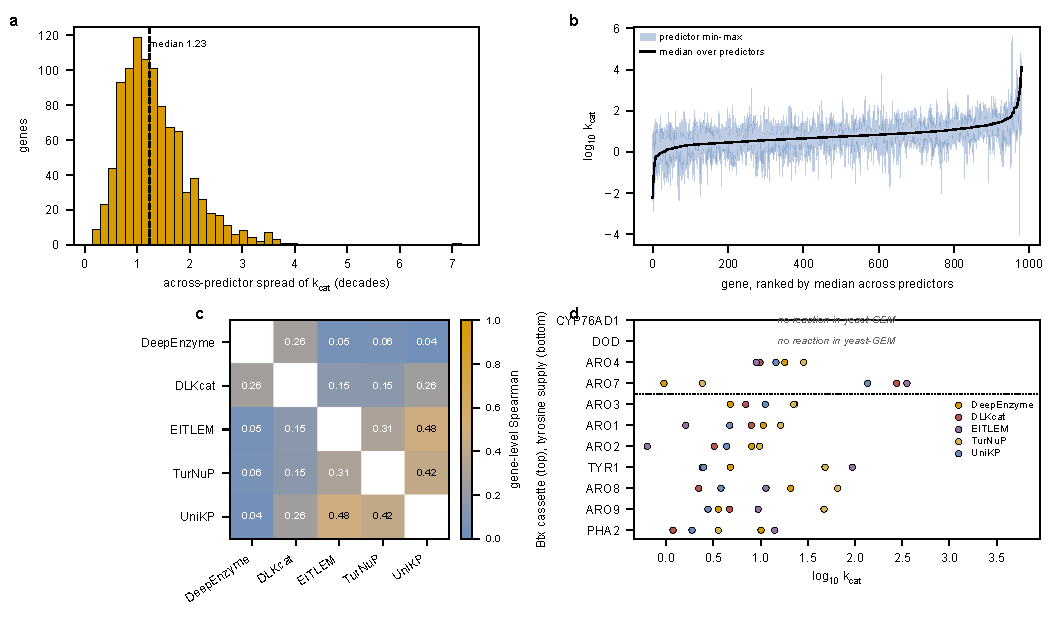
\includegraphics[width=\textwidth]{figures/per_gene_agreement_k_cat.pdf}
  \caption[Per-gene agreement between $k_{cat}$ predictors]{Agreement between the five
  $k_{cat}$ predictors at the level of a gene, over the 980 genes all five cover.
  \textbf{a}, Across-predictor spread per gene, the difference between the highest and
  lowest predictor in decades; the dashed line is the median, 1.23. \textbf{b}, The same
  spread against the dynamic range of $k_{cat}$ itself, genes ranked by their median across
  predictors: the band is the predictor min-max, the line the median. \textbf{c},
  Gene-level Spearman between predictors; the diagonal is left blank because a predictor
  against itself is 1 by construction. \textbf{d}, The genes the betaxanthin case study
  runs on. Above the dotted rule is the Btx cassette, below it the aromatic-amino-acid
  genes that supply its tyrosine precursor. \texttt{CYP76AD1} and \texttt{DOD} are
  heterologous and have no reaction in yeast-GEM, so no predictor emits a value for them.
  Generated by
  \texttt{experiments/026-metabolism-flux/scripts/plot\_per\_gene\_predictor\_agreement.py}.}
  \label{fig:per-gene}
\end{figure}

\textbf{For $k_{cat}$ the disagreement between predictors is larger than the quantity
being predicted.} The median gene moves 1.23 decades between the highest and lowest
predictor, a factor of 17, and 67 percent of genes move by more than a full decade. The
10th-to-90th-percentile range of the consensus estimate across genes is 0.94 decades. The
ratio is 1.32: choosing a different published predictor moves one gene's turnover number
further than real enzymes differ from one another. Panel b is that statement drawn, and the
band never narrows.

\textbf{For $K_M$ it is not.} The same construction over the three $K_M$ predictors gives a
median spread of 0.70 decades against a consensus range of 1.34, a ratio of 0.52, and
Boost\_KM agrees with UniKP at a gene-level Spearman of 0.75, higher than any pair of
$k_{cat}$ predictors reaches. Both facts are agreement rather than accuracy, since almost
none of these pairs has a measured value. Read that way they arrive at Wu et al.'s
conclusion from the other side: their claim is that underground metabolism separates from
known metabolism on $K_M$ rather than on $k_{cat}$, and $K_M$ is also the parameter the
instruments agree on well enough for a separation to be legible.

\textbf{The consequence for the flux layer.} An enzyme-constrained bound $v_j \le
k_{cat,j} E_j$ inherits panel a as its error bar, so a single predictor's table should not
be treated as the capacity constraint. The registry in
\texttt{torchcell/datasets/kinetics/} exists for that reason: predictor choice is a
hyperparameter with a measured effect size, not a settled detail.
